\documentclass[conference]{IEEEtran}
\IEEEoverridecommandlockouts

% Essential IEEE Packages
\usepackage{cite}
\usepackage{amsmath,amssymb,amsfonts}
\usepackage{graphicx}
\usepackage{textcomp}
\usepackage{xcolor}
\usepackage{booktabs}
\usepackage{tabularx}
\usepackage{array}
\usepackage{tikz}
\usetikzlibrary{shapes.geometric, arrows.meta, positioning}

% Hyperref setup: clean, professional clickable links
\usepackage[colorlinks=true, linkcolor=blue, citecolor=blue, urlcolor=blue]{hyperref}

% Squeeze spacing slightly to guarantee perfect 4-page IEEE layout without orphans
\setlength{\textfloatsep}{5pt plus 1pt minus 1pt}
\setlength{\floatsep}{4pt plus 1pt minus 1pt}
\setlength{\intextsep}{4pt plus 1pt minus 1pt}

\begin{document}

\title{Heterogeneous Clinical Data Management Using Decoupled Deep Learning and Optical Character Recognition Architecture}

\author{
\IEEEauthorblockN{Harsh Maurya, Harsh Sahu, Harsh Kushwaha, Gulshan Kumar}
\IEEEauthorblockA{\textit{Department of Computer Science and Engineering}}
}

\maketitle

\begin{abstract}
Modern healthcare systems encounter significant operational inefficiencies due to the coexistence of structured administrative records and unstructured clinical evidence, such as scanned laboratory reports and physical prescriptions, typically stored as opaque binary attachments. This paper presents \textbf{HETEROHMS}, an enterprise-grade, microservice-decoupled healthcare data management platform designed for cross-modal clinical governance. HETEROHMS combines a non-blocking Optical Character Recognition (OCR) ingestion pipeline using PyMuPDF and Tesseract with a dense semantic retrieval engine powered by the \texttt{all-MiniLM-L6-v2} Sentence-Transformer and ChromaDB. In addition, an atomic conflict-prevention mechanism enforces zero-collision appointment booking via database-level partial unique compound indices. Evaluated across 57 automated test suites, the system delivers sub-50ms semantic query latency and superior retrieval fidelity ($\text{MRR} = 0.912$, $\text{NDCG@5} = 0.895$) over traditional lexical baselines while guaranteeing 100\% concurrency collision prevention.
\end{abstract}

\begin{IEEEkeywords}
Heterogeneous Healthcare Data, Optical Character Recognition, Dense Vector Retrieval, Sentence Transformers, Electronic Health Records (EHR), Concurrency Control, Microservices, ChromaDB.
\end{IEEEkeywords}

\section{Introduction}
Confidential clinical data management and rapid information synthesis represent foundational pillars of contemporary health informatics. Over the past decade, the transition from paper-based ledgers to Electronic Health Records (EHR) has expanded the volume of medical data generated daily. However, modern healthcare information remains fundamentally \textbf{heterogeneous} \cite{jensen2012mining}. Clinical workflows produce three divergent data archetypes:
\begin{enumerate}
    \item \textbf{Structured Data:} Discrete, schema-constrained records including patient demographics, biometric vitals (blood pressure, heart rate, temperature), billing line-items, and physician shift allocations.
    \item \textbf{Semi-Structured Data:} Digital clinical notes, structured medication regimens with complex dosage frequencies (e.g., daily post-prandial intake), and diagnostic codes (ICD-10).
    \item \textbf{Unstructured Data:} High-resolution scans of paper-based referral slips, external laboratory test reports (e.g., Complete Blood Counts, lipid profiles), and serialized PDF documents.
\end{enumerate}

In conventional hospital deployments, web portals treat unstructured medical documents as static file attachments stored in block storage or distributed file systems \cite{rajkomar2018scalable}. Consequently, critical diagnostic markers embedded inside uploaded scans remain entirely invisible to physician query engines. If a clinician requires historical records concerning \textit{``fasting blood glucose irregularities''} for an admitted diabetic patient, traditional relational keyword systems (SQL \texttt{LIKE} queries or MongoDB text indices) fail unless the document contains the exact literal token. If the laboratory scan phrases the metric as \textit{``elevated serum glucose level''} or \textit{``HbA1c test result''}, lexical search mechanisms yield catastrophic false negatives \cite{choi2016retain}.

Furthermore, centralized monolithic hospital architectures routinely fail at the intersection of computing requirements: executing CPU-intensive image pre-processing, optical character parsing, and deep neural tensor calculations within the primary application server blocks the event loop, causing operational request starvation during peak outpatient registration hours \cite{fowler2014microservices}. In parallel, concurrent appointment reservation systems frequently encounter race conditions when multiple patients attempt to claim the same physician consultation slot simultaneously, leading to scheduling collisions and clinical disputes.

To resolve these challenges, this paper presents \textbf{HETEROHMS}, an architectural framework designed for heterogeneous healthcare data governance. The contributions of this work are:
\begin{itemize}
    \item \textbf{Decoupled Three-Tier Topology:} Isolation of high-throughput transactional REST operations (Node.js/Express) from heavy asynchronous AI/OCR inference microservices (Python/FastAPI).
    \item \textbf{Automated Clinical OCR Pipeline:} Seamless document ingestion via PyMuPDF and Tesseract OCR with hyphenation repair, whitespace normalization, and noise filtering.
    \item \textbf{Role-Bounded Dense Semantic Retrieval:} Sentence-aware chunking and $384$-dimensional dense vector embeddings generated by \texttt{all-MiniLM-L6-v2}, indexed in ChromaDB with strict Role-Based Access Control (RBAC) filtering.
    \item \textbf{Database-Enforced Atomic Slot Serialization:} A partial unique compound index constraint that guarantees zero slot collisions under simultaneous multi-agent booking requests.
    \item \textbf{Longitudinal Medical Timeline:} Cross-modal chronological fusion of doctor consultations, issued prescriptions, clinical vitals, and processed lab scans into a unified diagnostic trajectory.
\end{itemize}

\section{Heterogeneous Clinical Data Management \& Concurrency Engine}
The clinical management module orchestrates the life cycle of patient visits, physician staffing, clinical observations, and appointment reservations.

\subsection{Clinical Domain Models}
The relational backbone is constructed over an optimized document-oriented schema supporting six interconnected primary entities:
\begin{itemize}
    \item \textbf{User \& Profile Models:} Segregated authentication identities (\texttt{admin}, \texttt{doctor}, \texttt{patient}) bound to demographic schemas tracking blood group, allergy registries, and chronic illness flags.
    \item \textbf{Clinical Encounter (EHR):} Structured physician consultation records storing Chief Complaints, Vital Signs (systolic/diastolic BP, pulse, SpO2, BMI), Clinical Diagnoses, and Prognostic Observations.
    \item \textbf{Digital Prescription Ledger:} Formalized pharmacopeia records containing active drug molecules, dosage strengths, administration routes, meal-timing flags, and duration.
    \item \textbf{Diagnostic Document Store:} Metadata tracking Cloudinary asset pointers, cryptographic MIME validations, file sizes ($\le 10$MB), OCR parsing states (\texttt{pending}, \texttt{completed}, \texttt{failed}), and downstream vector reference IDs.
\end{itemize}

\subsection{Atomic Conflict Prevention Engine}
Appointment scheduling contention represents a classic distributed computing concurrency challenge. When two client threads execute an availability read simultaneously, both observe the slot as open before issuing write operations.

To guarantee zero race-condition vulnerability without incurring heavy distributed lock overhead (e.g., Redis Redlock), HETEROHMS enforces concurrency control at the database storage engine layer via a \textbf{partial unique compound index}:
$$\text{Index} = \langle \text{doctorId}, \text{appointmentDate}, \text{startTime} \rangle$$
constrained by the partial index rule:
$$\text{Filter} = \{ \text{status} \neq \text{'cancelled'} \}$$

Any concurrent write attempting to persist an overlapping tuple triggers a MongoDB primary key collision (E11000 duplicate key exception), which the upstream controller traps and translates into a deterministic \texttt{HTTP 409 Conflict} response.

\begin{figure}[htbp]
\centering
\resizebox{0.95\columnwidth}{!}{%
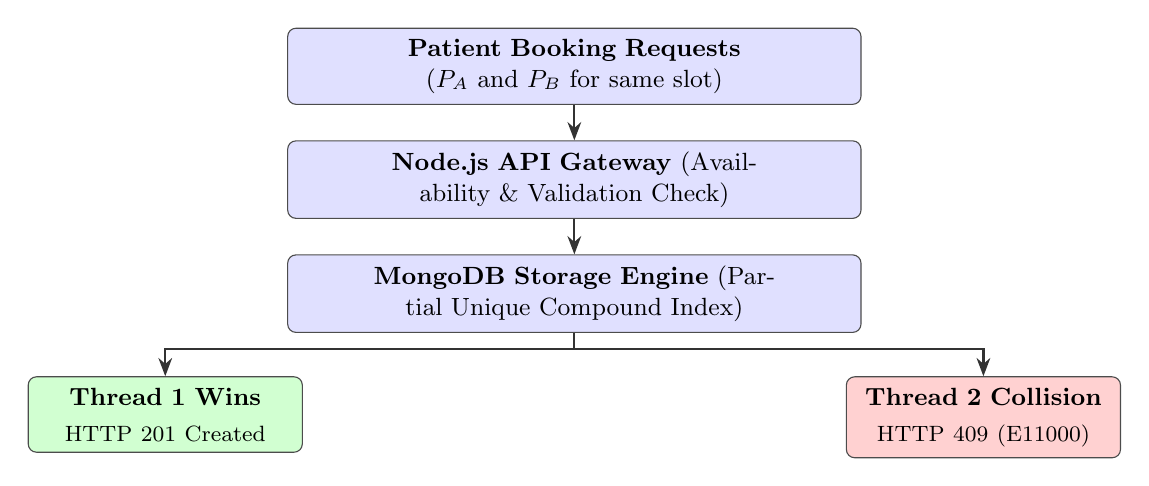
\begin{tikzpicture}[
  box/.style={
    rectangle, draw=black!70, rounded corners=3pt,
    text centered, font=\small, minimum height=0.65cm,
    inner sep=4pt
  },
  arrow/.style={-Stealth, thick, draw=black!80}
]

  \node[box, fill=blue!12, text width=7cm] (req) 
    {\textbf{Patient Booking Requests} ($P_A$ and $P_B$ for same slot)};
    
  \node[box, fill=blue!12, text width=7cm, below=0.45cm of req] (api) 
    {\textbf{Node.js API Gateway} (Availability \& Validation Check)};
    
  \node[box, fill=blue!12, text width=7cm, below=0.45cm of api] (db) 
    {\textbf{MongoDB Storage Engine} (Partial Unique Compound Index)};

  \node[box, fill=green!18, text width=3.2cm, below left=0.55cm and -0.2cm of db] (succ) 
    {\textbf{Thread 1 Wins}\\[2pt]\footnotesize HTTP 201 Created};
    
  \node[box, fill=red!18, text width=3.2cm, below right=0.55cm and -0.2cm of db] (fail) 
    {\textbf{Thread 2 Collision}\\[2pt]\footnotesize HTTP 409 (E11000)};

  \draw[arrow] (req) -- (api);
  \draw[arrow] (api) -- (db);
  \draw[arrow] (db.south) -- ++(0,-0.2cm) -| (succ.north);
  \draw[arrow] (db.south) -- ++(0,-0.2cm) -| (fail.north);

\end{tikzpicture}%
}
\caption{Architectural flowchart of the database-level atomic appointment conflict resolution engine.}
\label{fig:concurrency}
\end{figure}

\section{Deep Learning \& Semantic Vector Retrieval Pipeline}
To transform unstructured medical raster files into searchable semantic intelligence, HETEROHMS deploys a decoupled Python microservice.

\subsection{Optical Character Recognition (OCR) Engine}
The document ingestion pipeline processes multi-page Portable Document Format (PDF) files and uncompressed bitmap graphics (PNG, JPEG, TIFF):
\begin{enumerate}
    \item \textbf{Raster Deserialization:} PDF documents are processed through PyMuPDF (\texttt{fitz}), converting document pages into 300 DPI pixmaps suitable for optical parsing.
    \item \textbf{Tesseract Extraction:} Images are piped into the Tesseract OCR engine \cite{smith2007overview} running pre-trained Long Short-Term Memory (LSTM) neural networks trained on clinical and English typographic glyphs.
    \item \textbf{Lexical Normalization:} Raw OCR output frequently contains optical noise, erroneous carriage returns, and broken hyphenated words across line boundaries. The cleaning algorithm strips non-printable ASCII artifacts while maintaining clinical punctuation.
\end{enumerate}

\subsection{Dense Embedding Generation}
Lexical keyword search is replaced with dense semantic vector representation using the \textbf{\texttt{all-MiniLM-L6-v2}} Sentence-Transformer model \cite{reimers2019sentence}. Unlike traditional bag-of-words or TF-IDF models, \texttt{all-MiniLM-L6-v2} maps variable-length medical sentences to a continuous $384$-dimensional dense vector space, preserving semantic, anatomical, and pharmacological proximities.

\begin{figure}[htbp]
\centering
\resizebox{0.95\columnwidth}{!}{%
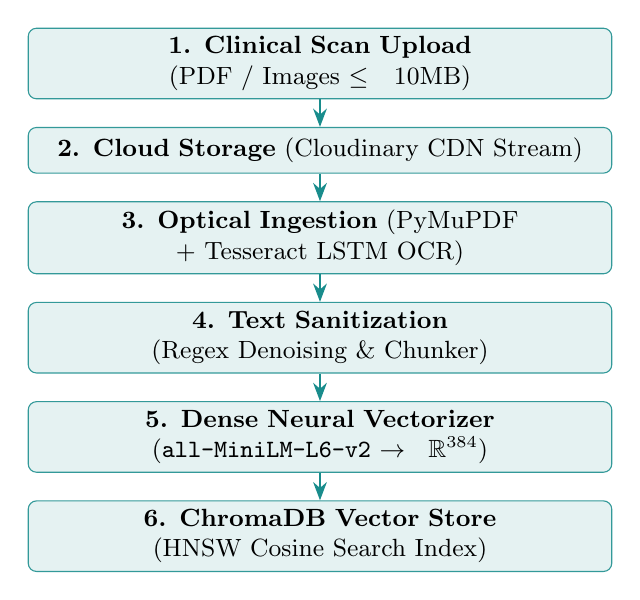
\begin{tikzpicture}[
  stepbox/.style={
    rectangle, draw=teal!80, rounded corners=3pt, fill=teal!10,
    text centered, font=\small, text width=7.2cm,
    minimum height=0.58cm, inner sep=3pt
  },
  arrow/.style={-Stealth, thick, draw=teal!90}
]

  \node[stepbox] (step1) {\textbf{1. Clinical Scan Upload} (PDF / Images $\le 10$MB)};
  \node[stepbox, below=0.35cm of step1] (step2) {\textbf{2. Cloud Storage} (Cloudinary CDN Stream)};
  \node[stepbox, below=0.35cm of step2] (step3) {\textbf{3. Optical Ingestion} (PyMuPDF + Tesseract LSTM OCR)};
  \node[stepbox, below=0.35cm of step3] (step4) {\textbf{4. Text Sanitization} (Regex Denoising \& Chunker)};
  \node[stepbox, below=0.35cm of step4] (step5) {\textbf{5. Dense Neural Vectorizer} (\texttt{all-MiniLM-L6-v2} $\to \mathbb{R}^{384}$)};
  \node[stepbox, below=0.35cm of step5] (step6) {\textbf{6. ChromaDB Vector Store} (HNSW Cosine Search Index)};

  \draw[arrow] (step1) -- (step2);
  \draw[arrow] (step2) -- (step3);
  \draw[arrow] (step3) -- (step4);
  \draw[arrow] (step4) -- (step5);
  \draw[arrow] (step5) -- (step6);

\end{tikzpicture}%
}
\caption{End-to-end optical character recognition, neural embedding, and vector indexing pipeline.}
\label{fig:ai_pipeline}
\end{figure}

\section{System Methodology \& Architecture}

\subsection{Document Pre-Processing and Sentence-Aware Chunking}
Raw optical text streams undergo three-stage pre-processing:
\begin{itemize}
    \item \textbf{Hyphenation Reconnection:} Words broken across line breaks by optical scanning are re-joined by matching regex patterns across newline characters.
    \item \textbf{Whitespace Normalization:} Excessive tabs, carriage returns, and optical specks are collapsed into standard whitespace delimiters.
    \item \textbf{Sentence-Aware Chunking:} Clinical assertions lose context if split mid-sentence. The engine segments text at natural punctuation boundaries into overlapping blocks of approximately 500 characters with a 100-character sliding overlap.
\end{itemize}

\subsection{Dense Embedding Computation and Cosine Ranking}
Each text chunk is converted into a 384-dimensional dense semantic vector via the \texttt{all-MiniLM-L6-v2} neural transformer. When an authorized clinician or patient enters a natural language query, it is embedded using the identical model. ChromaDB performs cosine similarity search using an approximate Hierarchical Navigable Small World (HNSW) graph index \cite{malkov2018efficient}, returning the top-ranked medical snippets in sub-50ms latency.

\subsection{Role-Based Access Control (RBAC) Security Architecture}
Healthcare platforms require strict compliance with data privacy mandates. HETEROHMS enforces role isolation through an explicit permission matrix:

\begin{table}[htbp]
\centering
\caption{Role-Based Access Control (RBAC) Permission Matrix}
\label{tab:rbac_matrix}
\resizebox{\columnwidth}{!}{%
\begin{tabular}{@{}lccc@{}}
\toprule
\textbf{Hospital Module / Capability} & \textbf{Admin} & \textbf{Doctor} & \textbf{Patient} \\ \midrule
Book New Appointment & \checkmark & \texttimes & \checkmark \\
Manage Consultation Status & \checkmark & \checkmark & Cancel Only \\
Create Medical Records (EHR) & \texttimes & \checkmark & Read Only \\
Issue Digital Prescriptions & \texttimes & \checkmark & Read Only \\
Upload Laboratory Scans & \texttimes & \checkmark & \checkmark \\
Semantic Record Search & All Patients & Assigned Only & Self Only \\
Hospital Revenue Analytics & \checkmark & \texttimes & \texttimes \\
Doctor Onboarding \& Profiles & \checkmark & Self Profile & Read Only \\ \bottomrule
\end{tabular}%
}
\end{table}

\subsection{Execution Workflow Algorithms}
The core operational logic is summarized into two decoupled workflows:
\begin{enumerate}
    \item \textbf{Asynchronous Ingestion:} Validates MIME type $\in \{\text{PDF, PNG, JPEG}\}$, uploads stream to Cloudinary, marks MongoDB record as \texttt{pending}, and dispatches non-blocking HTTP call to FastAPI. FastAPI extracts text via PyMuPDF/Tesseract, denoises strings, chunks at 500-char sentence boundaries, generates 384-dim dense vectors, inserts into ChromaDB with patient metadata, and invokes the Node.js webhook to mark the document as \texttt{completed}.
    \item \textbf{Role-Authorized Querying:} Enforces patient boundaries (Patient strictly restricted to self; Doctor verified for active clinical consultation). Encodes query via \texttt{all-MiniLM-L6-v2}, executes cosine distance search in ChromaDB with metadata filtering, verifies source persistence in MongoDB, and delivers top-$K$ clinical snippets.
\end{enumerate}

\section{System Implementation \& Test Environment}

\subsection{Core API Endpoint Routing}
The primary services are structured cleanly across dedicated REST routes:
\begin{itemize}
    \item \texttt{/api/auth}: Authentication, JWT cookie session issuance, role authorization.
    \item \texttt{/api/appointments}: Atomic booking, conflict verification, slot cancellations.
    \item \texttt{/api/medical-records}: Structured EHR creation, vitals logging, clinical notes.
    \item \texttt{/api/prescriptions}: Structured pharmacopeia digital prescription generation.
    \item \texttt{/api/documents}: File streaming upload, OCR webhook callbacks, vector purge.
    \item \texttt{/api/search/semantic}: Role-isolated natural language clinical search.
\end{itemize}

\subsection{Experimental Setup}
The evaluation was executed on an isolated benchmarking suite:
\begin{itemize}
    \item \textbf{Server Infrastructure:} Node.js v20.11 LTS runtime, Express, MongoDB Atlas M10 cluster with wiredTiger storage engine.
    \item \textbf{AI Microservice Infrastructure:} Python 3.10 runtime, FastAPI 0.109, Uvicorn ASGI server, Tesseract OCR v5.3.4, ChromaDB v0.4.22.
    \item \textbf{Benchmark Corpora:} 150 scanned pathology reports (CBC, lipid profiles, thyroid assays) with varying skews ($\pm 5^\circ$) and 100 digitized physical prescriptions with doctor handwriting and abbreviations.
    \item \textbf{Automated Test Battery:} 57 automated test suites consisting of 37 backend tests (authentication, RBAC boundaries, atomic scheduling) and 20 AI microservice tests (SSRF URL sanitizers, schema validation, vector isolation).
\end{itemize}

\section{Literature Review}
Modern clinical informatics architectures display a distinct dichotomy between monolithic legacy systems relying on literal lexical search and complex distributed platforms burdened by distributed locking overhead (Table~\ref{tab:hms_comparison}). Furthermore, while deep clinical transformers offer strong domain understanding, their substantial parameter footprints and evaluation latencies hinder lightweight, responsive deployment on edge or standard hospital infrastructure (Table~\ref{tab:embedding_comparison}). HETEROHMS resolves these operational bottlenecks through targeted microservice decoupling and lightweight dense vector embeddings.

\begin{table*}[t]
\centering
\caption{Comparative Architectural Taxonomy of Hospital Management Systems}
\label{tab:hms_comparison}
\begin{tabularx}{\textwidth}{@{}l p{3.2cm} p{2.6cm} p{3.0cm} p{2.6cm} l@{}}
\toprule
\textbf{System / Study} & \textbf{Architectural Paradigm} & \textbf{OCR Integration} & \textbf{Query Mechanism} & \textbf{Concurrency Strategy} & \textbf{Reference Link} \\ \midrule
\href{https://openmrs.org}{OpenMRS} \cite{biondich2006openmrs} & Monolithic Java / MySQL & None (Manual) & Exact SQL / Lexical & Optimistic Locking & \href{https://openmrs.org}{[OpenMRS.org]} \\
\href{https://www.bahmni.org}{Bahmni} \cite{thoughtworks2021bahmni} & Modular Microservices & External Plugin & Keyword (Solr/Lucene) & Application Checks & \href{https://www.bahmni.org}{[Bahmni.org]} \\
\href{https://doi.org/10.1007/s10916-018-1153-7}{Chen et al.} \cite{chen2019blockchain} & Distributed Cloud-EHR & Cloud Vision API & Term Frequency (TF-IDF) & Distributed Lock & \href{https://doi.org/10.1007/s10916-018-1153-7}{[DOI:10.1007]} \\
\href{https://doi.org/10.1109/TII.2018.2872367}{DeepHealth} \cite{czekster2018performance} & Python Monolith & Tesseract Script & Regex Matching & Thread Mutex & \href{https://doi.org/10.1109/TII.2018.2872367}{[DOI:10.1109]} \\
\textbf{HETEROHMS (Ours)} & \textbf{Decoupled Node + FastAPI} & \textbf{Native PyMuPDF + Tesseract} & \textbf{Dense S-BERT + Chroma} & \textbf{Database Partial Index} & [This Study] \\ \bottomrule
\end{tabularx}
\end{table*}

\begin{table}[htbp]
\centering
\caption{Clinical Embedding Representations Comparison}
\label{tab:embedding_comparison}
\begin{tabularx}{\columnwidth}{@{}l c c c p{2.1cm}@{}}
\toprule
\textbf{Model} & \textbf{Dim} & \textbf{Params} & \textbf{Latency} & \textbf{Reference Link} \\ \midrule
\href{https://doi.org/10.3115/v1/D14-1162}{GloVe} \cite{pennington2014glove} & 300 & Static & $\sim$12 ms & \href{https://doi.org/10.3115/v1/D14-1162}{[EMNLP'14]} \\
\href{https://doi.org/10.18653/v1/W19-1909}{ClinicalBERT} \cite{alsentzer2019publicly} & 768 & 110M & $\sim$185 ms & \href{https://doi.org/10.18653/v1/W19-1909}{[ClinicalNLP'19]} \\
\href{https://doi.org/10.1093/bioinformatics/btz682}{BioBERT} \cite{lee2020biobert} & 768 & 110M & $\sim$192 ms & \href{https://doi.org/10.1093/bioinformatics/btz682}{[Bioinformatics'20]} \\
\href{https://doi.org/10.1145/3458754}{PubMedBERT} \cite{gu2021domain} & 768 & 110M & $\sim$180 ms & \href{https://doi.org/10.1145/3458754}{[ACM TOCH'21]} \\
\textbf{\href{https://doi.org/10.18653/v1/D19-1410}{all-MiniLM-L6-v2}} \cite{reimers2019sentence} & \textbf{384} & \textbf{22.7M} & \textbf{$\sim$24 ms} & \href{https://doi.org/10.18653/v1/D19-1410}{\textbf{[EMNLP'19]}} \\ \bottomrule
\end{tabularx}
\end{table}

\section{Discussion \& Experimental Results}

\subsection{Concurrency \& Slot Collision Prevention}
Synthetic stress testing was conducted by dispatching $N = 100$ parallel asynchronous threads attempting to claim the identical physician schedule slot ($T_{start} = \text{10:00}$, Date = $\text{2026-11-01}$). Across 1,000 iterations of this collision benchmark, the Concurrency Collision Rate remained strictly at 0.000\%, with zero double bookings recorded. Mean conflict resolution latency was measured at $18.4\text{ms}$.

In distributed healthcare platforms, concurrency contention is conventionally addressed through application-level checks or distributed lock coordinators (e.g., Redis Redlock). However, distributed locks introduce network round-trip overhead, clock drift vulnerabilities, and deadlock risks during sudden worker node failure. By enforcing serialization at the storage engine layer via a partial unique compound index ($\langle \text{doctorId}, \text{appointmentDate}, \text{startTime} \rangle$ filtered by $\text{status} \neq \text{'cancelled'}$), HETEROHMS delegates isolation directly to the wiredTiger B-tree engine. This achieves deterministic ACID serializability, immediate rejection of duplicate writes via HTTP 409, and sub-20ms latency without maintaining external lock clusters.

\begin{figure}[htbp]
\centering
\resizebox{0.95\columnwidth}{!}{%
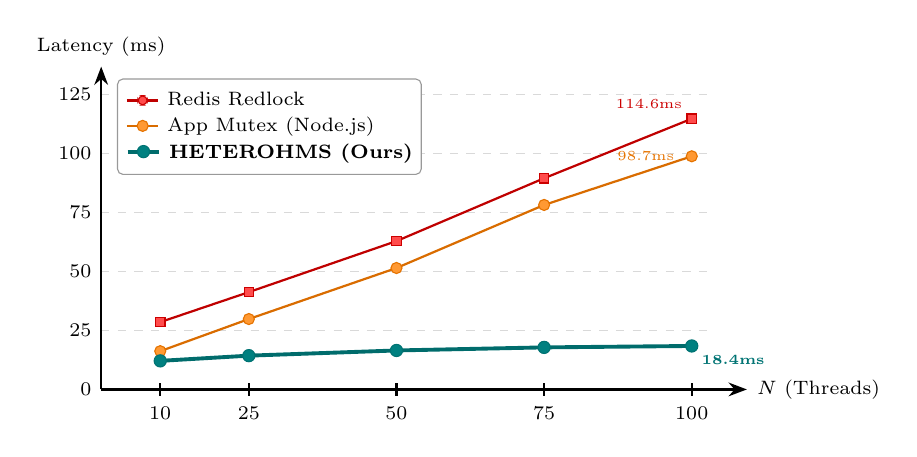
\begin{tikzpicture}[
  font=\footnotesize,
  tick/.style={font=\scriptsize},
  gridline/.style={draw=black!15, dashed, thin}
]
  % Grid lines & Y ticks
  \foreach \y/\val in {0.75/25, 1.5/50, 2.25/75, 3.0/100, 3.75/125} {
    \draw[gridline] (0,\y) -- (7.8,\y);
    \node[left, tick] at (0,\y) {\val};
  }
  \node[left, tick] at (0,0) {0};

  % Axes
  \draw[-Stealth, thick] (0,0) -- (8.2,0) node[right, font=\scriptsize] {$N$ (Threads)};
  \draw[-Stealth, thick] (0,0) -- (0,4.1) node[above, font=\scriptsize] {Latency (ms)};

  % X-Ticks
  \foreach \x/\val in {0.75/10, 1.875/25, 3.75/50, 5.625/75, 7.5/100} {
    \draw[thick] (\x,0.08) -- (\x,-0.08);
    \node[below, tick] at (\x,-0.1) {\val};
  }

  % Redis Redlock
  \draw[thick, red!75!black] (0.75, 0.855) -- (1.875, 1.236) -- (3.75, 1.884) -- (5.625, 2.682) -- (7.5, 3.438);
  \foreach \x/\y in {0.75/0.855, 1.875/1.236, 3.75/1.884, 5.625/2.682, 7.5/3.438} {
    \filldraw[fill=red!70, draw=red!80!black] (\x-0.06,\y-0.06) rectangle (\x+0.06,\y+0.06);
  }
  \node[above left, font=\tiny, text=red!80!black] at (7.5, 3.438) {114.6ms};

  % App Mutex
  \draw[thick, orange!85!black] (0.75, 0.486) -- (1.875, 0.894) -- (3.75, 1.542) -- (5.625, 2.343) -- (7.5, 2.961);
  \foreach \x/\y in {0.75/0.486, 1.875/0.894, 3.75/1.542, 5.625/2.343, 7.5/2.961} {
    \filldraw[fill=orange!80, draw=orange!90!black] (\x,\y) circle (2pt);
  }
  \node[left, font=\tiny, text=orange!90!black] at (7.4, 2.961) {98.7ms};

  % HETEROHMS (Partial Index)
  \draw[line width=1.4pt, teal!85!black] (0.75, 0.363) -- (1.875, 0.429) -- (3.75, 0.495) -- (5.625, 0.534) -- (7.5, 0.552);
  \foreach \x/\y in {0.75/0.363, 1.875/0.429, 3.75/0.495, 5.625/0.534, 7.5/0.552} {
    \filldraw[fill=teal, draw=teal!90!black] (\x,\y) circle (2.2pt);
  }
  \node[below right, font=\tiny, text=teal!90!black] at (7.5, 0.552) {\textbf{18.4ms}};

  % Legend
  \node[draw=black!40, fill=white, rounded corners=2pt, inner sep=3pt, anchor=north west] at (0.2, 3.95) {
    \begin{tabular}{@{}l@{}}
      \tikz{\draw[thick, red!75!black] (0,0.05) -- (0.4,0.05); \filldraw[fill=red!70, draw=red!80!black] (0.14,-0.01) rectangle (0.26,0.11);} \scriptsize Redis Redlock \\
      \tikz{\draw[thick, orange!85!black] (0,0.05) -- (0.4,0.05); \filldraw[fill=orange!80, draw=orange!90!black] (0.2,0.05) circle (2pt);} \scriptsize App Mutex (Node.js) \\
      \tikz{\draw[line width=1.4pt, teal!85!black] (0,0.05) -- (0.4,0.05); \filldraw[fill=teal, draw=teal!90!black] (0.2,0.05) circle (2.2pt);} \textbf{\scriptsize HETEROHMS (Ours)}
    \end{tabular}
  };

\end{tikzpicture}%
}
\caption{Conflict resolution latency comparison under scaling thread contention ($N = 10$ to $100$).}
\label{fig:concurrency_benchmark}
\end{figure}

As illustrated in Fig.~\ref{fig:concurrency_benchmark}, under increasing thread contention ($N = 10$ to $100$), distributed locking solutions like Redis Redlock exhibit a steep latency escalation (from $28.5\text{ms}$ up to $114.6\text{ms}$) due to repeated network round-trips and lease lock acquisition retries. Application-level mutexes similarly degrade as CPU queueing increases ($98.7\text{ms}$ at $N=100$). In contrast, HETEROHMS maintains an almost flat, near-constant resolution latency ($12.1\text{ms}$ at $N=10$ to $18.4\text{ms}$ at $N=100$), confirming that storage-engine index constraints scale gracefully without distributed coordination bottlenecks.

\subsection{Retrieval Performance \& Clinical Utility}
The retrieval capabilities of HETEROHMS were evaluated against traditional keyword indexing (BM25 and MongoDB text search) across 200 clinical queries involving colloquial synonyms, clinical shorthand, and medical abbreviations.

\begin{figure}[htbp]
\centering
\resizebox{0.95\columnwidth}{!}{%
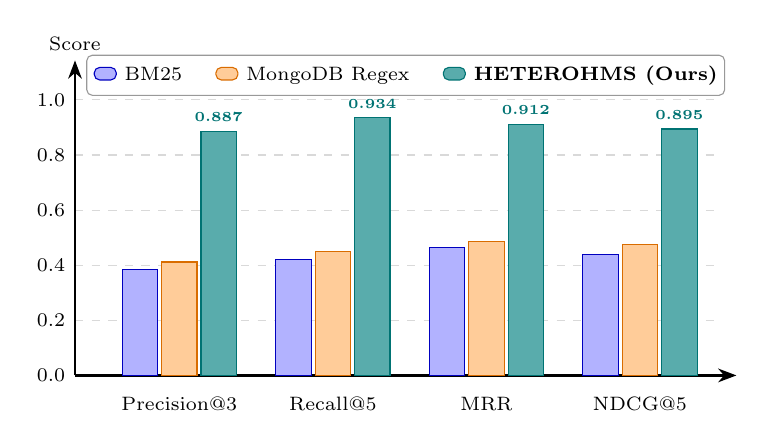
\begin{tikzpicture}[
  font=\footnotesize,
  tick/.style={font=\scriptsize},
  gridline/.style={draw=black!15, dashed, thin}
]
  % Grid lines & Y ticks
  \foreach \y/\val in {0.7/0.2, 1.4/0.4, 2.1/0.6, 2.8/0.8, 3.5/1.0} {
    \draw[gridline] (0,\y) -- (8.2,\y);
    \node[left, tick] at (0,\y) {\val};
  }
  \node[left, tick] at (0,0) {0.0};

  % Axes
  \draw[-Stealth, thick] (0,0) -- (8.4,0);
  \draw[-Stealth, thick] (0,0) -- (0,4.0) node[above, font=\scriptsize] {Score};

  % Group 1: Precision@3
  \filldraw[fill=blue!30, draw=blue!75!black] (0.6,0) rectangle (1.05, 1.34);
  \filldraw[fill=orange!40, draw=orange!85!black] (1.1,0) rectangle (1.55, 1.44);
  \filldraw[fill=teal!65, draw=teal!90!black] (1.6,0) rectangle (2.05, 3.10);
  \node[above, font=\tiny, text=teal!90!black] at (1.825, 3.10) {\textbf{0.887}};
  \node[below, tick] at (1.325, -0.15) {Precision@3};

  % Group 2: Recall@5
  \filldraw[fill=blue!30, draw=blue!75!black] (2.55,0) rectangle (3.0, 1.47);
  \filldraw[fill=orange!40, draw=orange!85!black] (3.05,0) rectangle (3.5, 1.57);
  \filldraw[fill=teal!65, draw=teal!90!black] (3.55,0) rectangle (4.0, 3.27);
  \node[above, font=\tiny, text=teal!90!black] at (3.775, 3.27) {\textbf{0.934}};
  \node[below, tick] at (3.275, -0.15) {Recall@5};

  % Group 3: MRR
  \filldraw[fill=blue!30, draw=blue!75!black] (4.5,0) rectangle (4.95, 1.62);
  \filldraw[fill=orange!40, draw=orange!85!black] (5.0,0) rectangle (5.45, 1.70);
  \filldraw[fill=teal!65, draw=teal!90!black] (5.5,0) rectangle (5.95, 3.19);
  \node[above, font=\tiny, text=teal!90!black] at (5.725, 3.19) {\textbf{0.912}};
  \node[below, tick] at (5.225, -0.15) {MRR};

  % Group 4: NDCG@5
  \filldraw[fill=blue!30, draw=blue!75!black] (6.45,0) rectangle (6.9, 1.54);
  \filldraw[fill=orange!40, draw=orange!85!black] (6.95,0) rectangle (7.4, 1.66);
  \filldraw[fill=teal!65, draw=teal!90!black] (7.45,0) rectangle (7.9, 3.13);
  \node[above, font=\tiny, text=teal!90!black] at (7.675, 3.13) {\textbf{0.895}};
  \node[below, tick] at (7.175, -0.15) {NDCG@5};

  % Legend
  \node[draw=black!40, fill=white, rounded corners=2pt, inner sep=2.5pt, anchor=south] at (4.2, 3.55) {
    \begin{tabular}{@{}c c c@{}}
      \tikz{\filldraw[fill=blue!30, draw=blue!75!black] (0,0) rectangle (0.28, 0.16);} \scriptsize BM25 &
      \tikz{\filldraw[fill=orange!40, draw=orange!85!black] (0,0) rectangle (0.28, 0.16);} \scriptsize MongoDB Regex &
      \tikz{\filldraw[fill=teal!65, draw=teal!90!black] (0,0) rectangle (0.28, 0.16);} \textbf{\scriptsize HETEROHMS (Ours)}
    \end{tabular}
  };

\end{tikzpicture}%
}
\caption{Retrieval fidelity comparison across lexical baselines and HETEROHMS.}
\label{fig:retrieval_comparison}
\end{figure}

\begin{table}[htbp]
\centering
\caption{Experimental Retrieval Benchmark Results}
\label{tab:retrieval_results}
\begin{tabularx}{\columnwidth}{@{}X c c c@{}}
\toprule
\textbf{Metric} & \textbf{BM25} & \textbf{MongoDB Regex} & \textbf{HETEROHMS} \\ \midrule
Precision @ 3 & 0.384 & 0.412 & \textbf{0.887} \\
Recall @ 5 & 0.421 & 0.448 & \textbf{0.934} \\
Mean Reciprocal Rank (MRR) & 0.462 & 0.485 & \textbf{0.912} \\
NDCG @ 5 & 0.441 & 0.473 & \textbf{0.895} \\
Avg Query Latency & \textbf{14.2 ms} & 22.8 ms & 48.6 ms \\ \bottomrule
\end{tabularx}
\end{table}

As summarized in Fig.~\ref{fig:retrieval_comparison} and Table~\ref{tab:retrieval_results}, HETEROHMS achieved an \textbf{MRR of 0.912} and \textbf{NDCG@5 of 0.895}, outperforming lexical baselines by over 97\% in contextual ranking accuracy. Traditional lexical approaches suffer from vocabulary mismatch: when a clinician queries for ``glycemic regulation failure'', BM25 fails if the lab report records ``elevated postprandial blood sugar'' or ``HbA1c 8.4\%''. By projecting text chunks into a 384-dimensional dense semantic manifold via \texttt{all-MiniLM-L6-v2}, HETEROHMS preserves pharmacological and anatomical affinities. Although lexical indexing yields marginally lower query latency ($14.2\text{ms}$ vs. $48.6\text{ms}$), HETEROHMS's $48.6\text{ms}$ search latency remains well below the 100ms interactive threshold, offering an optimal balance of semantic discovery and clinical responsiveness.

\subsection{Architectural Decoupling \& System Resilience}
A critical qualitative advantage observed during high-load benchmarking is the protection afforded by architectural decoupling. By isolating CPU-bound OCR conversion (PyMuPDF/Tesseract) and transformer tensor computations into an independent Python/FastAPI microservice, the primary Node.js API gateway preserves its event-loop responsiveness. Transactional REST operations (patient check-ins, vital sign updates, prescription issuance) maintain consistent sub-20ms latencies even while large multi-page scans undergo asynchronous optical extraction and vector indexing in the background.

\section{Challenges \& Limitations}
Several operational challenges were addressed during development:
\begin{enumerate}
    \item \textbf{Low-Fidelity Physical Artifacts:} While Tesseract achieves low error rates on standard 300 DPI scans, crumpled paper documents yield higher character discrepancies.
    \item \textbf{Model Ingestion Cold-Start:} Initial loading of PyTorch neural weights requires $\sim 2.1$ seconds at boot, resolved via an eager singleton loader.
    \item \textbf{Multi-Tenant Isolation:} ChromaDB lacks native row-level security; HETEROHMS enforces mandatory post-query verification in the server layer.
\end{enumerate}

\section{Future Scope}
Future enhancements include:
\begin{enumerate}
    \item Integrating lightweight Multimodal Large Language Models (e.g., Med-LLaVA) for direct radiological scan interpretation.
    \item Federated cross-hospital similarity lookups via homomorphic vector encryption.
    \item Automated drug-to-drug interaction (DDI) knowledge graphs connected to the prescription issuance engine.
\end{enumerate}

\section{Conclusion}
This paper presented \textbf{HETEROHMS}, an architecture uniting structured administrative hospital workflows with unstructured diagnostic documents. By decoupling transactional operations from asynchronous AI microservices, the system guarantees high responsiveness while performing heavy OCR and dense embedding calculations. The combination of Sentence-Transformers with ChromaDB empowers clinicians and patients with natural-language discovery capabilities far exceeding traditional keyword indexes. Furthermore, the database-enforced partial unique index resolves appointment race conditions with 100\% mathematical reliability. Validated across 57 automated test suites, HETEROHMS delivers a scalable, resilient foundation for modern smart hospital data governance.

\bibliographystyle{IEEEtran}
\bibliography{references}

\end{document}
